
%(BEGIN_QUESTION)
% Copyright 2006, Tony R. Kuphaldt, released under the Creative Commons Attribution License (v 1.0)
% This means you may do almost anything with this work of mine, so long as you give me proper credit

Her vises mekanismen for en forenklet pneumatisk regulator med kun proporsjonalvirkning (ingen forsterkerrelé, ingen bias-fjær):

$$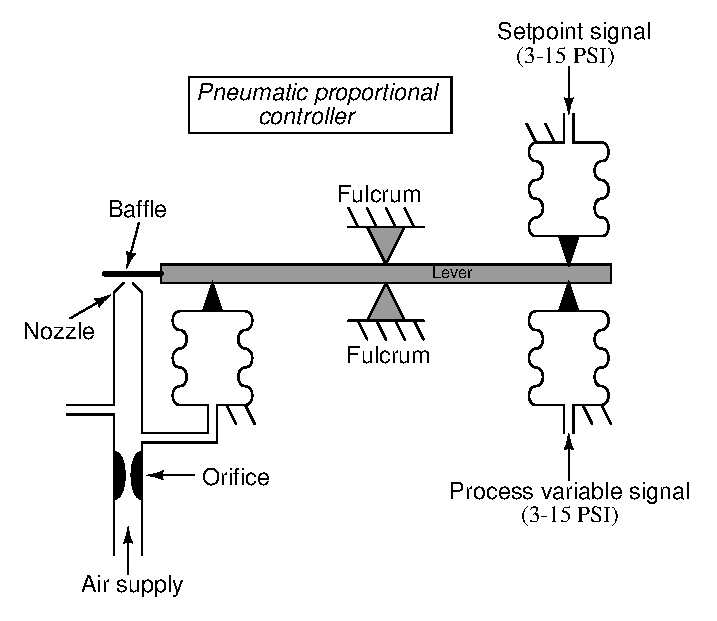
\includegraphics[width=15.5cm]{i01596x01.eps}$$

Hva må endres eller justeres i denne mekanismen for å {\it redusere} regulatorens proporsjonalbånd? Bestem også om denne regulatoren er {\it direktevirkende} eller {\it reversvirkende}.

\vskip 20pt \vbox{\hrule \hbox{\strut \vrule{} {\bf Forslag til sokratisk diskusjon} \vrule} \hrule}

\begin{itemize}
\item{} Er dette en {\it kraftbalanse}-mekanisme eller en {\it bevegelsesbalanse}-mekanisme? Hvordan kan du vite det sikkert?
\item{} Kan mekanismen endres slik at den blir den andre typen balanse? Hvis ja, hvordan?
\end{itemize}

\underbar{file i01596}
%(END_QUESTION)





%(BEGIN_ANSWER)

For å redusere regulatorens proporsjonalbånd (øke forsterkningen), flytt vippepunktet lenger mot venstre:

$$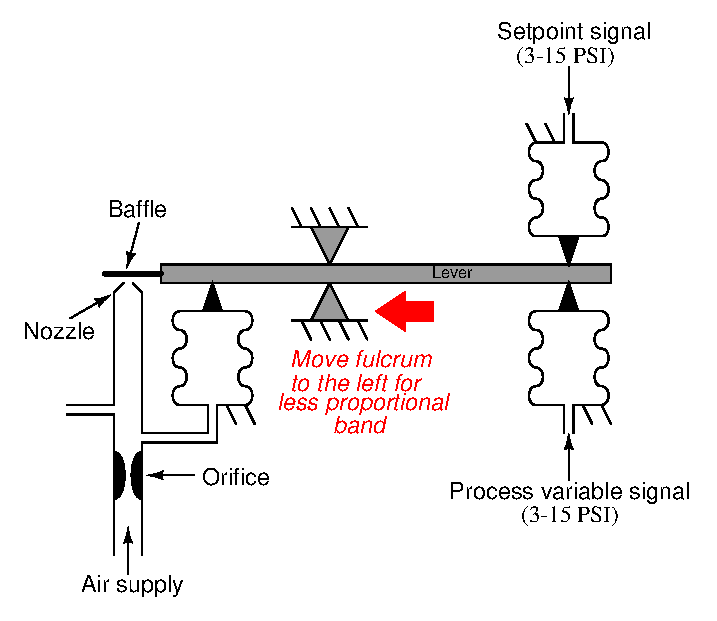
\includegraphics[width=15.5cm]{i01596x02.eps}$$

Denne regulatormekanismen er direktevirkende.

%(END_ANSWER)





%(BEGIN_NOTES)

Når vippepunktet flyttes mot venstre, må utgangsbelgen reagere mer aggressivt på endringer i avvik (PV $-$ SP), fordi kraften virker over en kortere momentarm. Dette tilsvarer økt forsterkning, som er det samme som redusert proporsjonalbånd.

Noen studenter kan tro det motsatte, fordi de ser at en flytting av vippepunktet mot venstre reduserer baffelbevegelsen relativt til dysen, og dermed tror at utgangsresponsen blir mindre. Dette er riktig når vi ser på bevegelse, men ikke riktig når vi ser på {\it kraft}. Siden mekanismen er kraftbalanse og ikke bevegelsesbalanse, må vi tenke i krefter.

Et tankeeksperiment som ofte fjerner denne misforståelsen, er å forestille seg at tilbakekoblingsbelgen ikke finnes. Hvis tilbakekoblingsbelgen ikke var der, ville plasseringen av vippepunktet i det hele tatt hatt betydning? Selvsagt ikke, siden {\it ethvert} avvik ville presset baffelen langt nok til å nå metning i utgangen. Det er krafttilbakekoblingen som får denne regulatormekanismen til å virke, ikke den synlige bevegelsen.

Minn studentene på at en forsterket baffel/dyse-enhet bare trenger å bevege seg noen få tusendels tomme for å nå full utgangsmetning!

%INDEX% Control, proportional: pneumatic force-balance controller

%(END_NOTES)
